\documentclass[10pt]{beamer}

% Packages
\usepackage[utf8]{inputenc}
\usepackage[T1]{fontenc}
\usepackage{amsmath, amssymb, amsthm}
\usepackage{graphicx}
\usepackage{booktabs}
\usepackage{hyperref}
\usepackage{tikz}
\usetikzlibrary{shapes,arrows,positioning,calc}

% Theme settings
\usetheme{default}
\usecolortheme{default}
\usefonttheme{professionalfonts}

\definecolor{ImperialBlue}{RGB}{0, 62, 116}
\definecolor{DarkGray}{RGB}{51, 51, 51}
\definecolor{LightGray}{RGB}{245, 245, 245}
\definecolor{AccentOrange}{RGB}{214, 96, 77}
\definecolor{AccentGreen}{RGB}{46, 139, 87}

% Apply colors
\setbeamercolor{frametitle}{fg=ImperialBlue, bg=white}
\setbeamercolor{title}{fg=ImperialBlue}
\setbeamercolor{structure}{fg=ImperialBlue}
\setbeamercolor{normal text}{fg=DarkGray}
\setbeamercolor{block title}{fg=white, bg=ImperialBlue}
\setbeamercolor{block body}{fg=DarkGray, bg=LightGray}
\setbeamercolor{itemize item}{fg=ImperialBlue}
\setbeamercolor{enumerate item}{fg=ImperialBlue}

% Remove navigation symbols
\setbeamertemplate{navigation symbols}{}

% Customize frame title
\setbeamertemplate{frametitle}{
  \vspace{0.5em}
  \insertframetitle
  \vspace{0.3em}
}

% Customize itemize
\setbeamertemplate{itemize items}[circle]
\setlength{\leftmargini}{1.5em}

% Footer
\setbeamertemplate{footline}{
  \leavevmode%
  \hbox{%
  \begin{beamercolorbox}[wd=.333333\paperwidth,ht=2.25ex,dp=1ex,left]{author in head/foot}%
    \hspace{1em}\usebeamerfont{author in head/foot}\insertshortauthor
  \end{beamercolorbox}%
  \begin{beamercolorbox}[wd=.333333\paperwidth,ht=2.25ex,dp=1ex,center]{title in head/foot}%
    \usebeamerfont{title in head/foot}\insertshorttitle
  \end{beamercolorbox}%
  \begin{beamercolorbox}[wd=.333333\paperwidth,ht=2.25ex,dp=1ex,right]{date in head/foot}%
    \usebeamerfont{date in head/foot}\insertshortdate{}\hspace*{2em}
    \insertframenumber{} / \inserttotalframenumber\hspace*{2ex} 
  \end{beamercolorbox}}%
  \vskip0pt%
}

% Commands for highlighting
\newcommand{\emphbox}[1]{\colorbox{LightGray}{\textcolor{DarkGray}{#1}}}
\newcommand{\highlight}[1]{\textcolor{AccentOrange}{\textbf{#1}}}
\newcommand{\good}[1]{\textcolor{AccentGreen}{#1}}
\newcommand{\bad}[1]{\textcolor{AccentOrange}{#1}}

%----------------------------------------------------------------------------------------
\title{Cryptocurrencies as an Asset Class (Part I)}
\subtitle{ECOM215: Blockchain Economics and Digital Assets}
\author{Dr Daniele Bianchi}
\institute{Queen Mary, University of London}
\date{Semester B, 2025/2026}
%----------------------------------------------------------------------------------------

\begin{document}

\AtBeginSection[]{
  \begin{frame}[plain]
    \vfill
    \begin{center}
      {\Large\color{ImperialBlue}\insertsection}
    \end{center}
    \vfill
  \end{frame}
}

\begin{frame}[plain]
  \titlepage
\end{frame}

\begin{frame}{Today's Agenda}
  \tableofcontents
\end{frame}

%----------------------------------------------------------------------------------------
\section{From Technology to Investment}
%----------------------------------------------------------------------------------------

\begin{frame}{Where We Are in the Course}
  \textbf{Weeks 1--6}: We studied the \highlight{technology} and its \highlight{applications}.
  \begin{itemize}
    \item How blockchains work (consensus, cryptography, smart contracts)
    \item What you can build on them (DeFi, stablecoins, tokenized assets)
    \item What can go wrong (Terra/Luna, smart contract exploits, oracle failures)
  \end{itemize}
  
  \vspace{1em}
  \textbf{Weeks 7--8}: Now we ask a different question:
  
  \vspace{0.5em}
  \begin{center}
    \Large Should anyone \highlight{invest} in these things?
  \end{center}
  
  \vspace{1em}
  This requires a shift in perspective---from engineering and protocol design to \textbf{financial economics}: returns, risk, valuation, market structure, and portfolio construction.
\end{frame}

\begin{frame}{The Two Big Questions}
  \textbf{This lecture:} Is cryptocurrency a legitimate asset class?
  \begin{itemize}
    \item How do crypto markets actually work?
    \item Can we value these assets?
    \item What are the risk-return characteristics?
  \end{itemize}
  
  \vspace{1em}
  \textbf{Next lecture:} How do investors access crypto?
  \begin{itemize}
    \item The 2024 spot ETF approvals and their implications
    \item Institutional adoption and custody
    \item Investment vehicles (direct and indirect)
    \item Market integrity and manipulation risks
  \end{itemize}
  
  \vspace{1em}
  \begin{block}{Approach}
    We apply standard asset pricing intuition throughout. Crypto is not a special universe---it either meets the criteria we apply to any investment, or it doesn't.
  \end{block}
\end{frame}

%----------------------------------------------------------------------------------------
\section{What Makes an Asset Class?}
%----------------------------------------------------------------------------------------

\begin{frame}{Asset Class: Definition and Criteria}
  An \highlight{asset class} is a group of investments with similar characteristics, subject to similar economic forces and regulatory treatment.
  
  \vspace{1em}
  \textbf{Four criteria} for evaluating any asset class:
  \begin{enumerate}
    \item \textbf{Return potential}: What drives returns? Are they compensation for risk?
    \item \textbf{Risk characteristics}: Volatility, tail risk, drawdowns
    \item \textbf{Liquidity}: Can you trade at scale without moving the price?
    \item \textbf{Regulatory framework}: Is there investor protection? Legal clarity?
  \end{enumerate}
  
  \vspace{1em}
  A fifth consideration for portfolio construction:
  \begin{itemize}
    \item \textbf{Correlation structure}: Does the asset provide diversification?
  \end{itemize}
  
  \vspace{0.5em}
  We will evaluate cryptocurrencies against each of these criteria. The answer is not straightforward.
\end{frame}

\begin{frame}{Where Do Cryptocurrencies Fit?}
  Cryptocurrencies are typically classified as \highlight{alternative investments}, alongside hedge funds, private equity, real estate, and commodities.
  
  \vspace{1em}
  But the analogy is imperfect:
  \begin{itemize}
    \item Unlike real estate or commodities, most cryptoassets \textbf{generate no cash flows}
    \item Unlike hedge funds or PE, there is \textbf{no fund manager} making allocation decisions
    \item Unlike gold, the ``store of value'' narrative is \textbf{contested and empirically fragile}
    \item Unlike equities, there are \textbf{no earnings, dividends, or buybacks} to anchor valuation
  \end{itemize}
  
  \vspace{1em}
  \begin{block}{Key Tension}
    The institutional investment case for crypto rests on (i) attractive risk-adjusted returns and (ii) low correlation with traditional assets. We will examine the evidence for both claims.
  \end{block}
\end{frame}

%----------------------------------------------------------------------------------------
\section{Crypto Market Structure}
%----------------------------------------------------------------------------------------

\begin{frame}{How Crypto Markets Work: An Overview}
  Crypto markets differ from traditional financial markets in several fundamental ways:
  
  \vspace{1em}
  \begin{columns}[T]
    \column{0.48\textwidth}
    \textbf{Traditional equities:}
    \begin{itemize}
      \item Centralised exchanges (NYSE, LSE)
      \item Regulated market makers
      \item Consolidated tape (one price)
      \item Trading hours (9:30--16:00)
      \item T+1 settlement
      \item Regulated custody (broker-dealer)
    \end{itemize}
    
    \column{0.48\textwidth}
    \textbf{Cryptocurrency:}
    \begin{itemize}
      \item Multiple venues (CEX + DEX)
      \item Unregulated or lightly regulated
      \item No consolidated tape (fragmented)
      \item 24/7/365 trading
      \item Near-instant or on-chain settlement
      \item Self-custody or third-party custodian
    \end{itemize}
  \end{columns}
  
  \vspace{1em}
  Each of these differences creates both \good{opportunities} and \bad{risks} for investors.
\end{frame}

\begin{frame}{Centralised Exchanges (CEXs)}
  \textbf{CEXs} are the dominant trading venues: Binance, Coinbase, Kraken, OKX, Bybit.
  
  \vspace{0.5em}
  \textbf{How they work:}
  \begin{itemize}
    \item Traditional limit order book model (similar to stock exchanges)
    \item The exchange holds custody of user funds (``not your keys, not your coins'')
    \item Matching engine pairs buy and sell orders
    \item Revenue from trading fees (typically 0.01\%--0.60\% per trade)
  \end{itemize}
  
  \vspace{0.5em}
  \textbf{Key risks:}
  \begin{itemize}
    \item \textbf{Counterparty risk}: Exchange insolvency (FTX, 2022) or hacks (Mt.\ Gox, 2014)
    \item \textbf{Commingling}: Some exchanges mix customer and proprietary funds
    \item \textbf{Regulatory arbitrage}: Many exchanges operate from loosely regulated jurisdictions
  \end{itemize}
  
  % \vspace{0.5em}
  % % FIGURE PLACEHOLDER: Monthly spot trading volume across major CEXs (stacked bar chart)
  % % Source: The Block (theblock.co) — "Cryptocurrency Exchange Volume (Monthly)"
  % % Suggested update: Use data through 2025
  % \textit{[Figure: Monthly spot trading volume across major CEXs. Source: theblock.co]}
\end{frame}

\begin{frame}{Centralised Exchanges (CEXs)}
  \begin{figure}
    \centering
    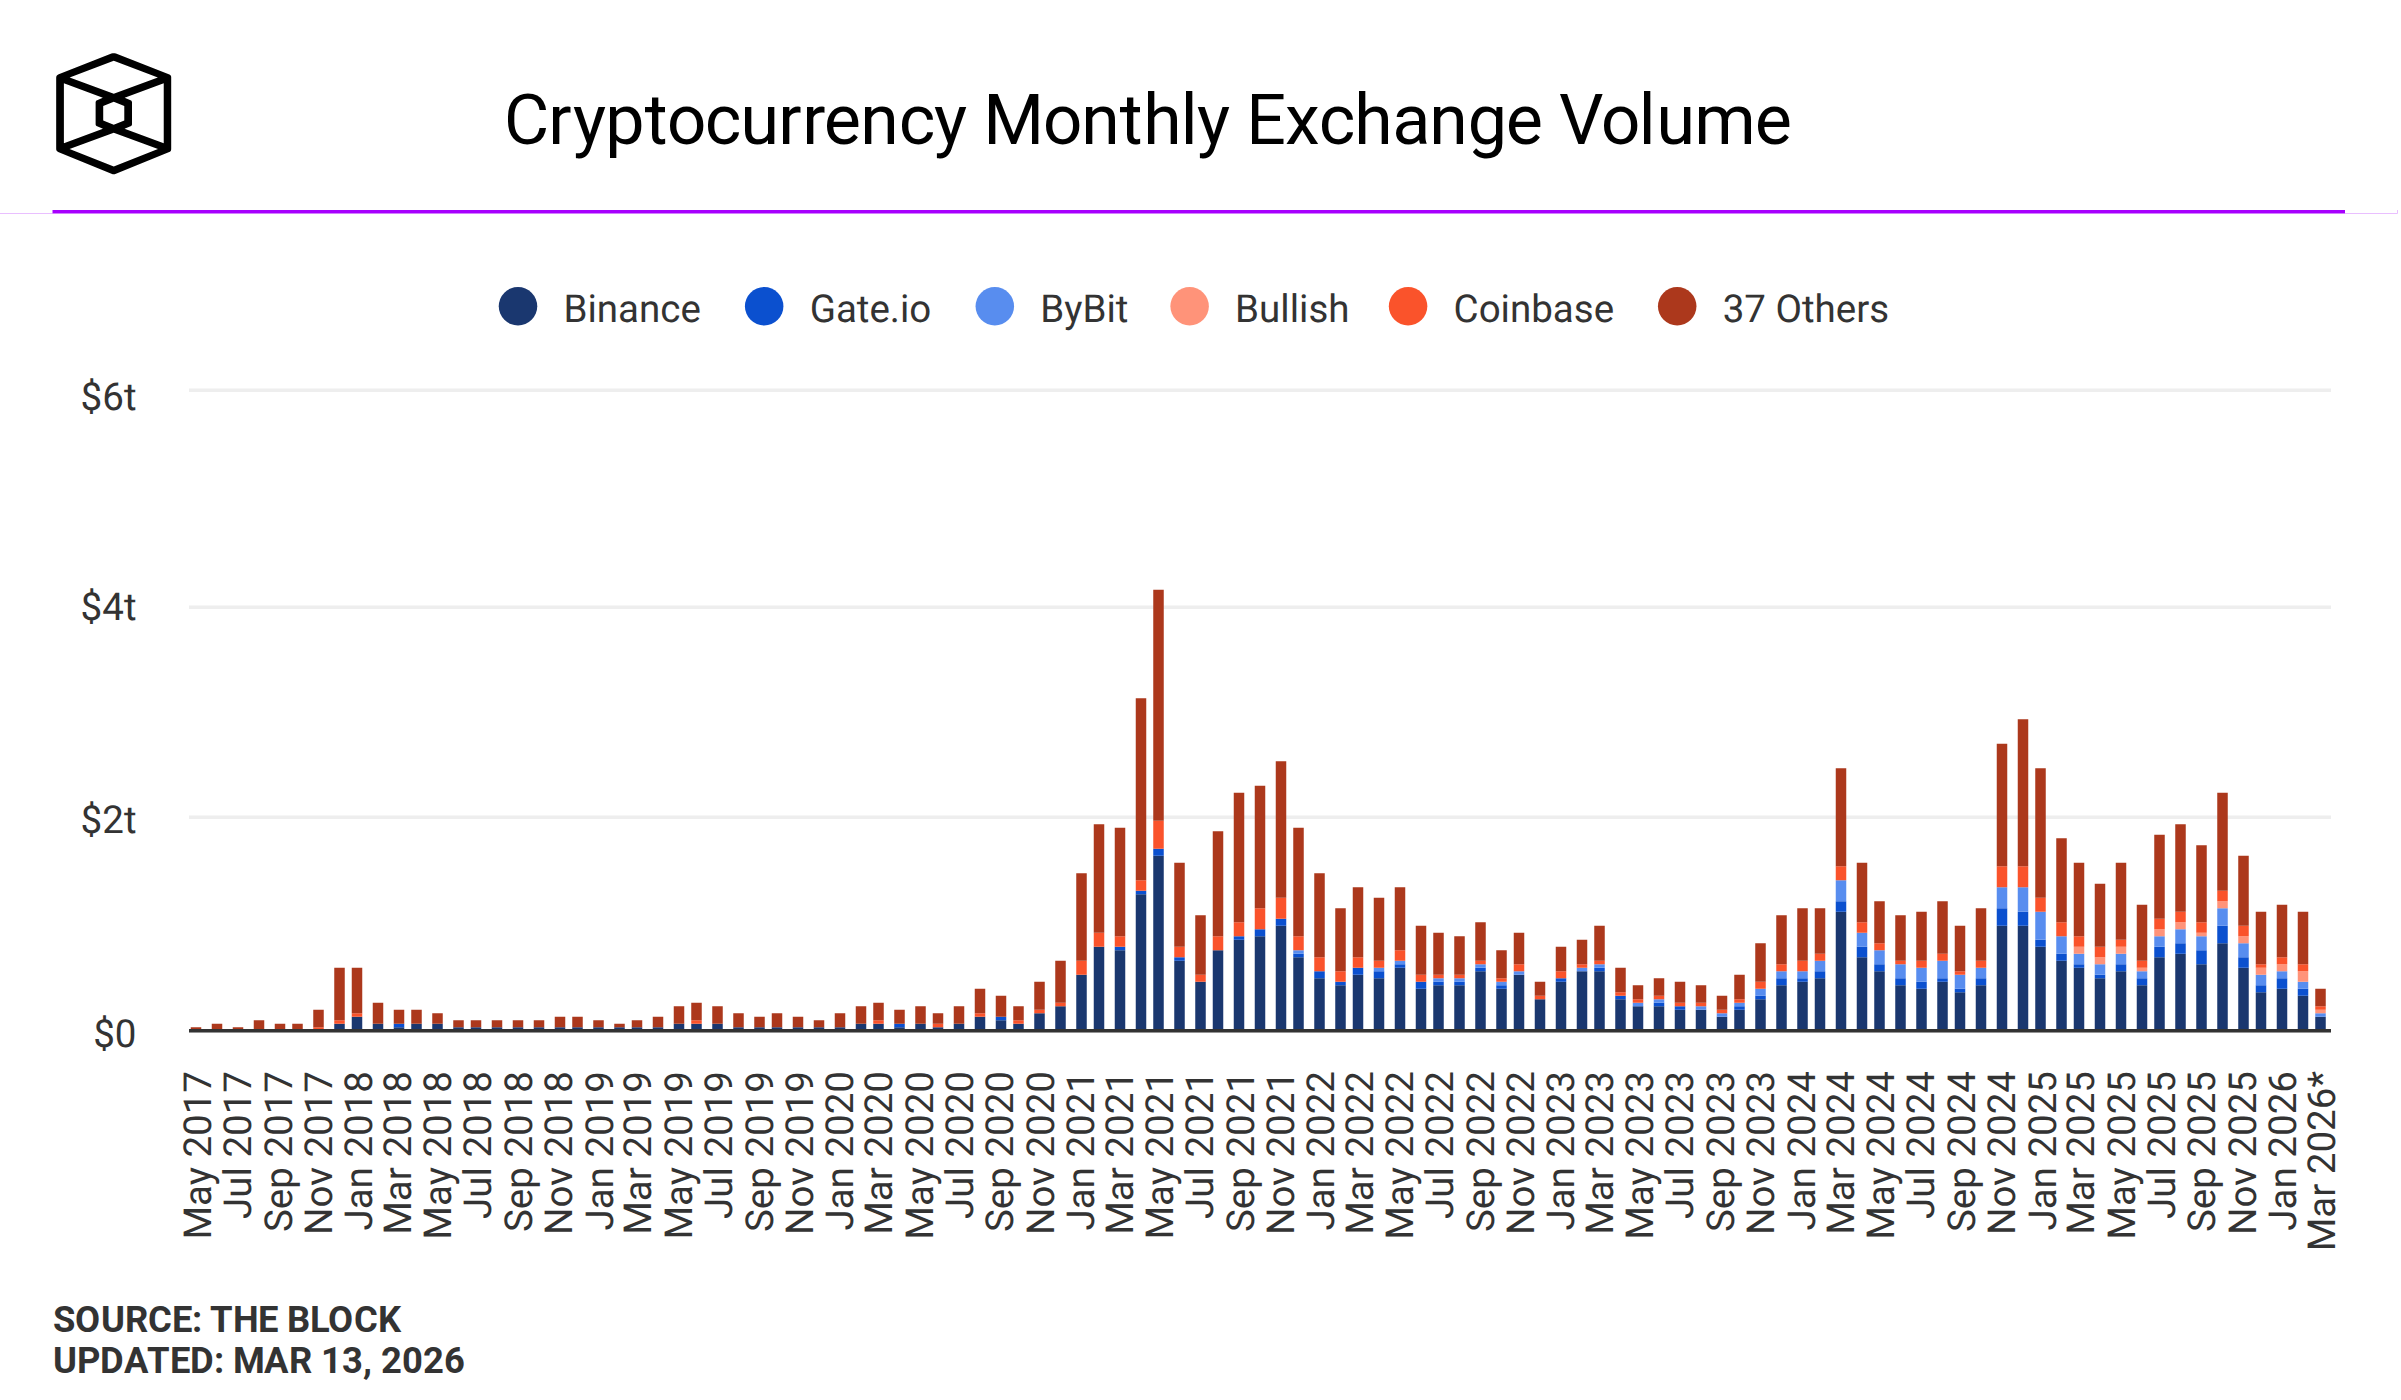
\includegraphics[width=1\linewidth]{Figures/cryptocurrency-exchange-volume-monthly.png}
    \caption{Monthly spot trading volume across major CEXs. Source: theblock.co}
    \label{fig:CEX volume}
  \end{figure}
\end{frame}


\begin{frame}{Decentralised Exchanges (DEXs)}
  \textbf{DEXs} use the AMM model we studied in Week 4 (Uniswap, Curve, etc.)
  
  \vspace{0.5em}
  \textbf{Key differences from CEXs:}
  \begin{itemize}
    \item No centralised order book---liquidity pools and automated pricing
    \item Non-custodial: users retain control of their assets (connect wallet, trade, disconnect)
    \item Transparent: all trades visible on-chain
    \item Permissionless: anyone can list a token (which is also a risk)
  \end{itemize}
  
  \vspace{0.5em}
  \textbf{Market share:} DEXs account for approximately 15--20\% of total spot volume, growing but still far behind CEXs.
  
  \vspace{0.5em}
  \textbf{Economic trade-off:}
  \begin{itemize}
    \item \good{No counterparty risk} (no exchange can freeze your funds)
    \item \bad{Higher costs} for large trades (slippage, gas fees)
    \item \bad{Smart contract risk} replaces counterparty risk
  \end{itemize}
  
  % \vspace{0.5em}
  % % FIGURE PLACEHOLDER: DEX vs CEX spot trading volume over time
  % % Source: The Block — "DEX to CEX Spot Trade Volume (%)"
  % \textit{[Figure: DEX vs.\ CEX spot trade volume ratio over time. Source: theblock.co]}
\end{frame}

\begin{frame}{Decentralised Exchanges (DEXs)}
 \begin{figure}
    \centering
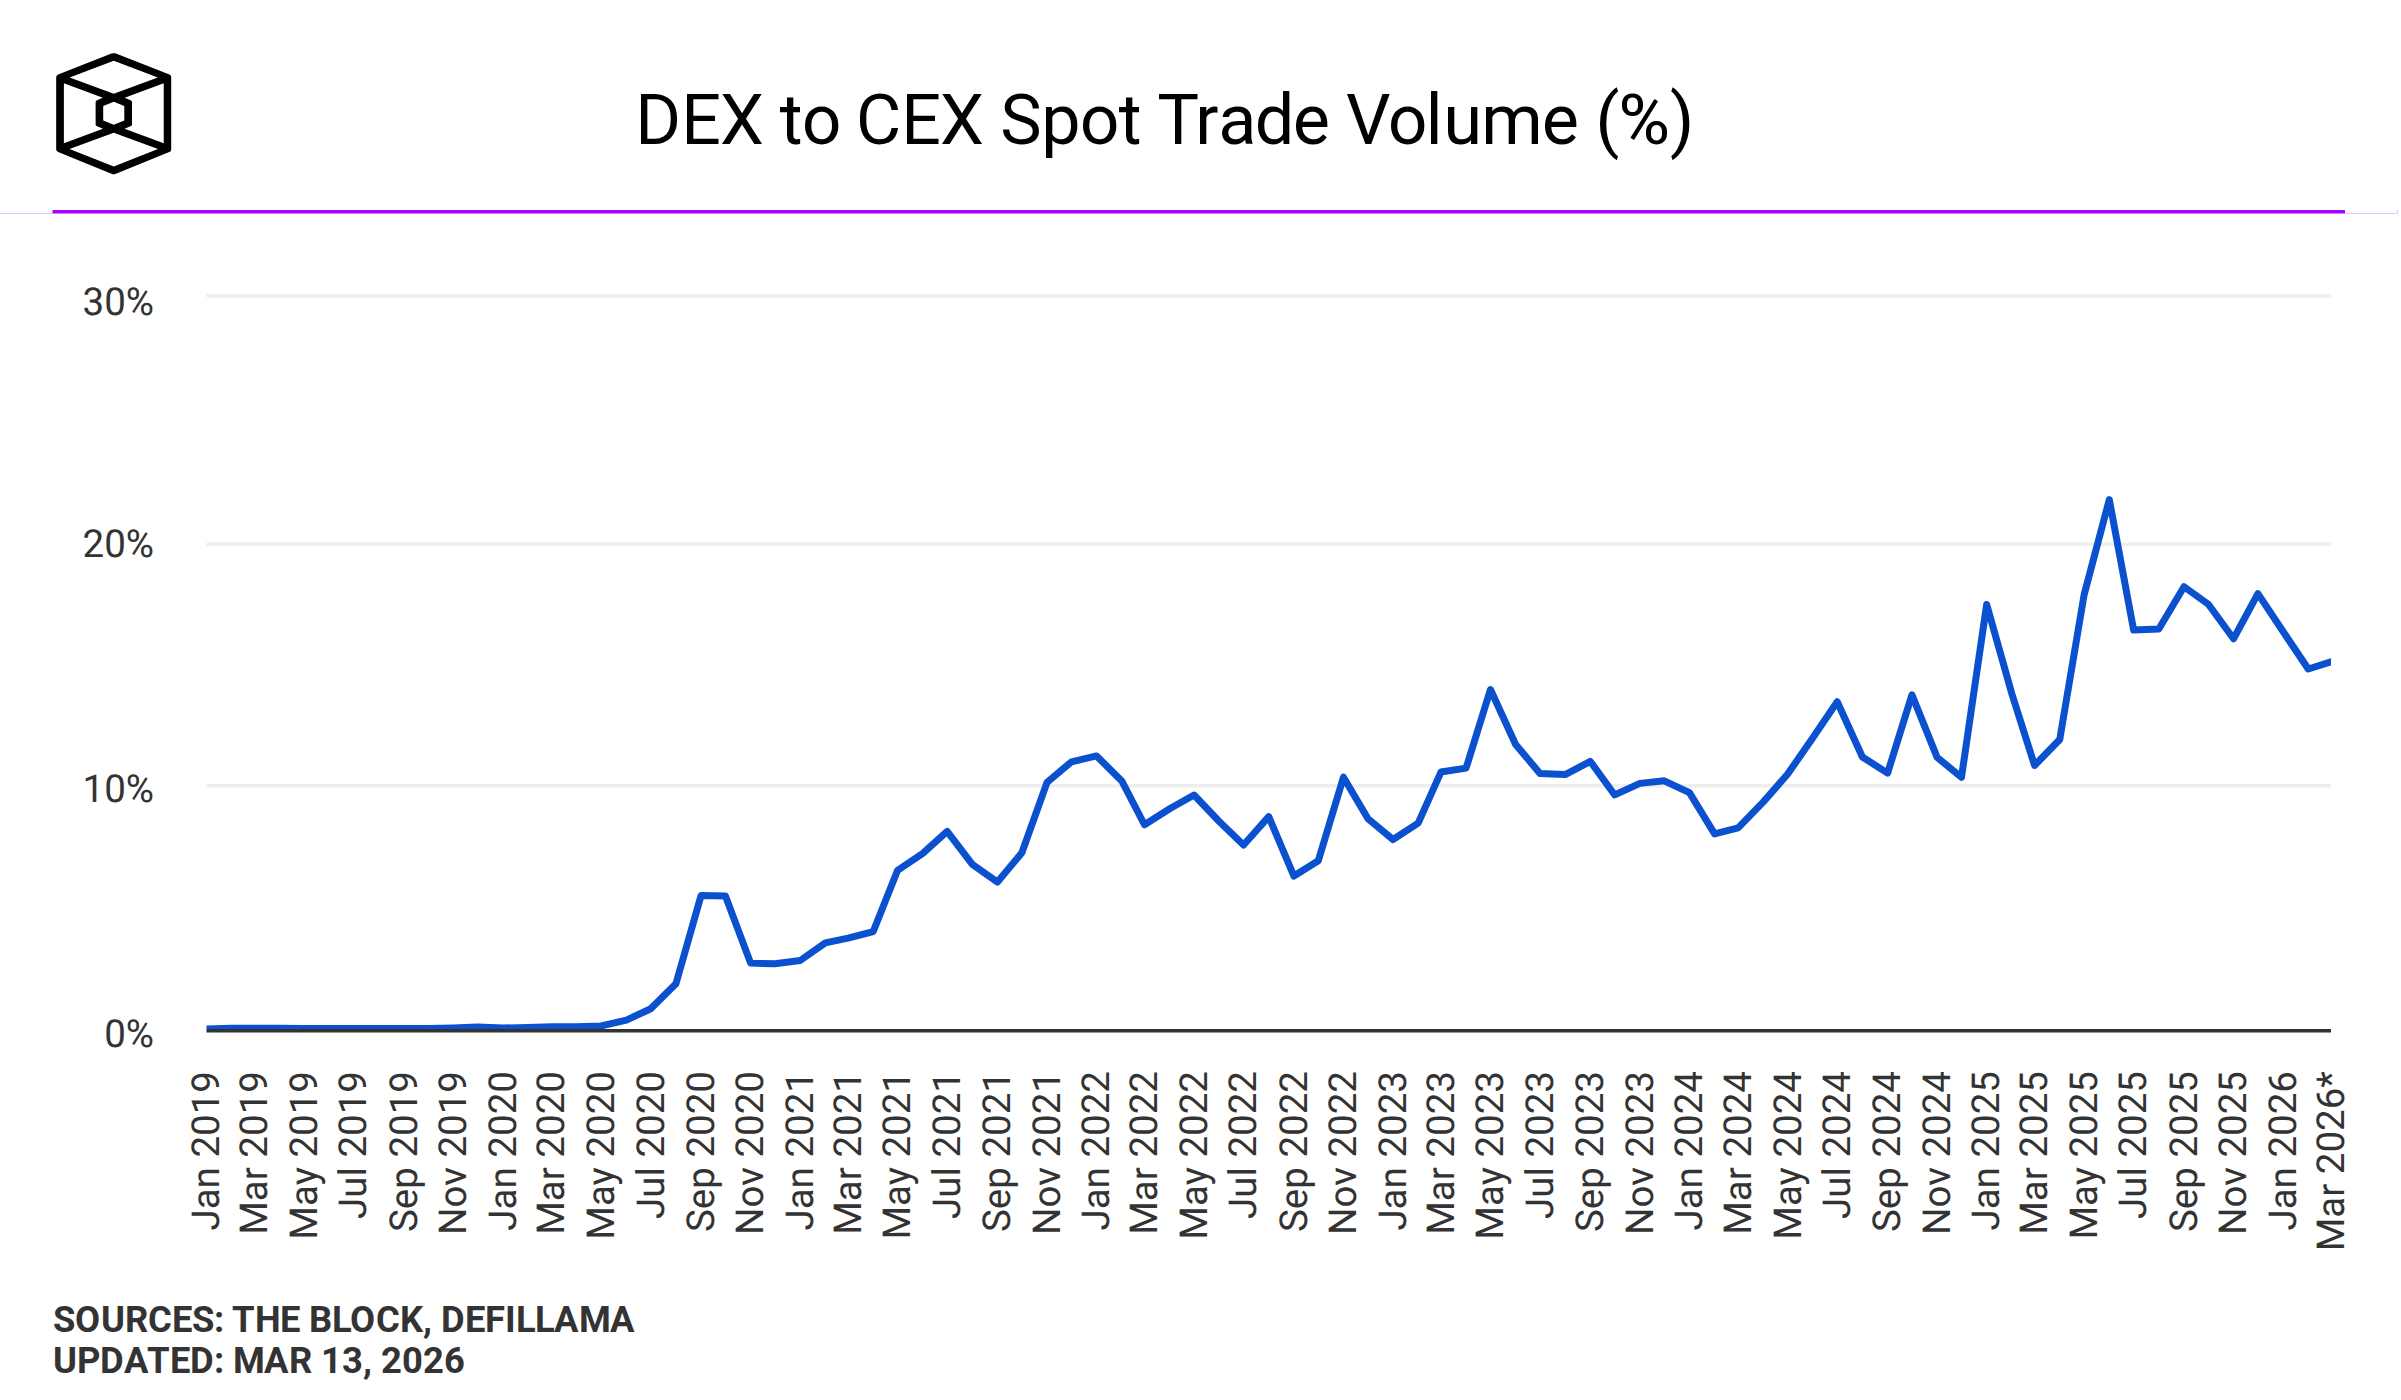
\includegraphics[width=1\linewidth]{Figures/dex-to-cex-spot-trade-volume.png}
\caption{DEX vs.\ CEX spot trade volume ratio over time. Source: theblock.co}
    \label{fig:CEX vs DEX volume}
\end{figure}
\end{frame}



\begin{frame}{Market Fragmentation and Price Discovery}
  Unlike equities, there is \highlight{no consolidated tape} for crypto prices.
  
  \vspace{0.5em}
  \textbf{What this means:}
  \begin{itemize}
    \item The ``price of Bitcoin'' depends on which exchange you look at
    \item Price differences across venues create arbitrage opportunities
    \item Arbitrageurs link prices across exchanges, but not perfectly
  \end{itemize}
  
  \vspace{0.5em}
  \textbf{Consequences for investors:}
  \begin{itemize}
    \item \textbf{Execution quality varies}: Different price on different venues
    \item \textbf{Reference price ambiguity}: Which price do ETFs, futures, and indices use?
    \item \textbf{Manipulation risk}: Easier to manipulate price on a single venue when there is no consolidated reference
  \end{itemize}
  
  % \vspace{0.5em}
  % \begin{block}{Comparison}
  %   In equity markets, the National Best Bid and Offer (NBBO) ensures investors get the best available price across all exchanges. No equivalent exists for crypto.
  % \end{block}
\end{frame}

\begin{frame}{Liquidity: Bid-Ask Spreads and Slippage}
  Liquidity determines how cheaply and quickly you can trade.
  
  \vspace{0.5em}
  \textbf{Two key measures:}
  \begin{itemize}
    \item \textbf{Bid-ask spread}: The gap between the best buy and sell price. Tighter spreads = more liquid market.
    \item \textbf{Slippage}: How much the execution price moves against you for a given order size. Relevant for institutional-sized trades.
  \end{itemize}
  
  \vspace{0.5em}
  \textbf{Crypto liquidity stylised facts:}
  \begin{itemize}
    \item BTC and ETH on major exchanges: spreads comparable to mid-cap equities
    \item Altcoins: spreads can be 10--100$\times$ wider
    \item Liquidity evaporates during stress events (``liquidity illusion'')
    \item 24/7 trading means liquidity varies by time of day and day of week
  \end{itemize}
  
  % \vspace{0.5em}
  % % FIGURE PLACEHOLDER: Two-panel figure
  % % Left: Bid-ask spreads (BTC/USD, bps) across major exchanges
  % % Right: Slippage for $100k sell order (BTC/USD, bps) across major exchanges
  % % Source: Kaiko via The Block
  % \textit{[Figure: Bid-ask spreads and slippage costs across major exchanges. Source: Kaiko via theblock.co]}
\end{frame}

\begin{frame}{Liquidity: Bid-Ask Spreads and Slippage}
 \begin{figure}
    \centering
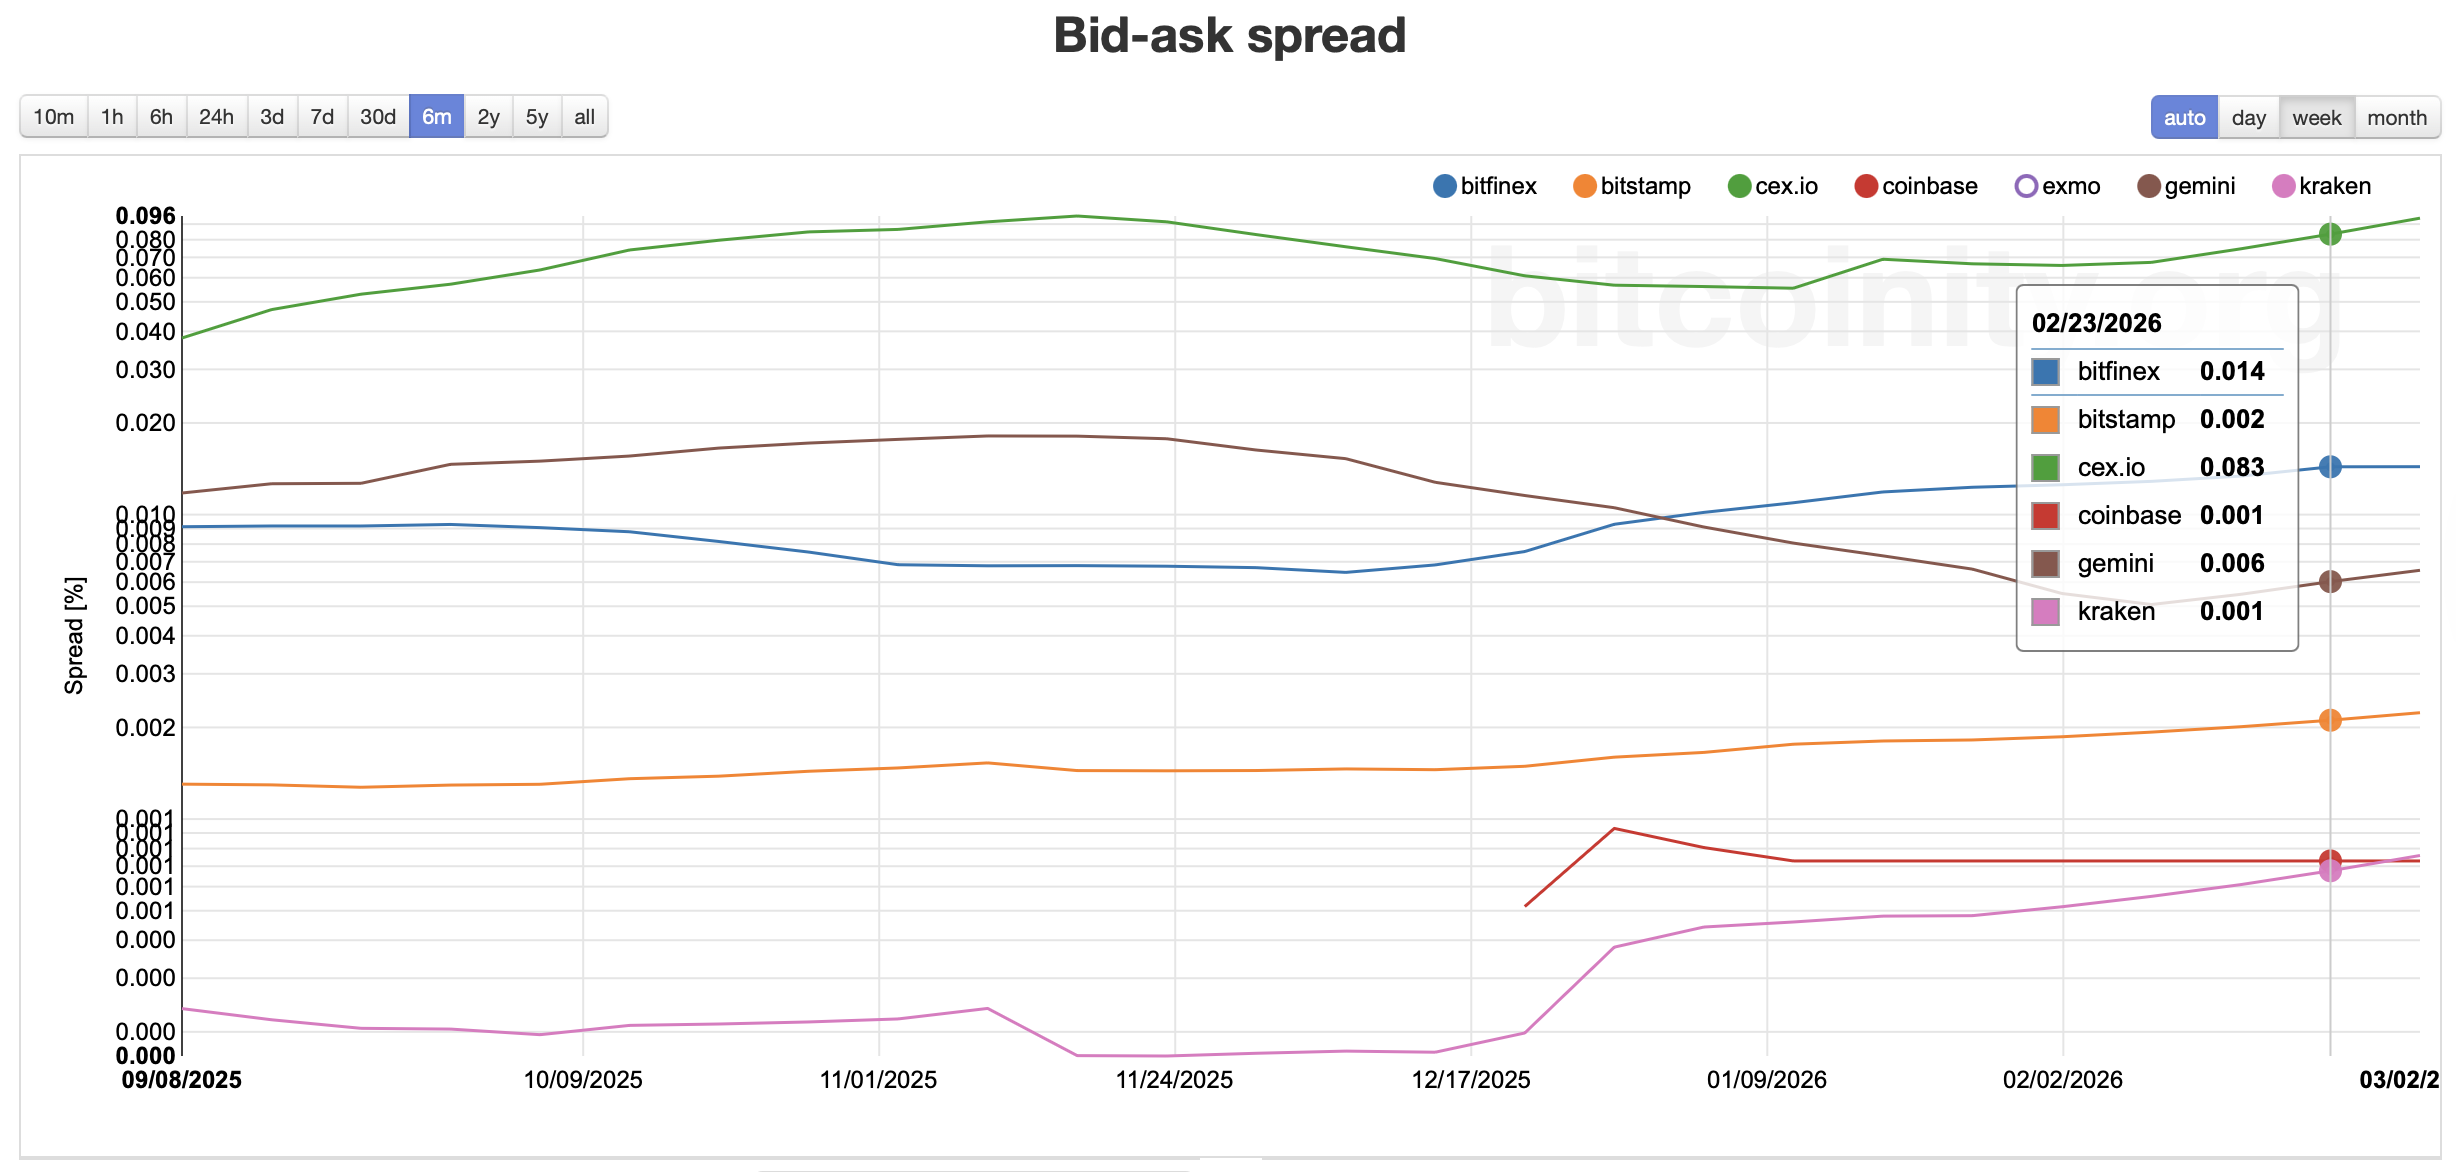
\includegraphics[width=1\linewidth]{Figures/bidask_bitcoin.png}
\caption{Bid-ask spreads and slippage costs across major exchanges. Source: Kaiko via theblock.co}
    \label{fig:bidask}
\end{figure}
\end{frame}

\begin{frame}{The Custody Problem}
  \textbf{Custody} = who holds the assets and how are they secured?
  
  \vspace{0.5em}
  In traditional finance, custody is a solved problem: regulated broker-dealers and custodian banks hold securities on behalf of investors, with legal protections and insurance.
  
  \vspace{0.5em}
  In crypto, custody is a \highlight{first-order risk}:
  
  \vspace{0.5em}
  \begin{columns}[T]
    \column{0.48\textwidth}
    \textbf{Self-custody:}
    \begin{itemize}
      \item User controls private keys
      \item No counterparty risk
      \item But: loss of keys = permanent loss of assets
      \item Not practical for institutions
    \end{itemize}
    
    \column{0.48\textwidth}
    \textbf{Third-party custody:}
    \begin{itemize}
      \item Coinbase Custody, Fidelity Digital Assets, BitGo
      \item Regulated qualified custodians
      \item Required for ETFs and institutional mandates
      \item Re-introduces counterparty risk
    \end{itemize}
  \end{columns}
  
  \vspace{0.5em}
  The development of \textbf{institutional-grade custody} was a prerequisite for the 2024 ETF approvals---the SEC needed assurance that the underlying Bitcoin was held securely. We will return to this in next lecture.
\end{frame}

%----------------------------------------------------------------------------------------
\section{The Valuation Problem}
%----------------------------------------------------------------------------------------

\begin{frame}{How Do You Value a Cryptocurrency?}
  \textbf{Traditional asset valuation} is grounded in \highlight{discounted cash flows}:
  \begin{itemize}
    \item Equities: Present value of expected dividends/earnings
    \item Bonds: Present value of coupon payments and principal
    \item Real estate: Present value of rental income
  \end{itemize}
  
  \vspace{1em}
  \textbf{The fundamental problem with most cryptoassets:}
  
  \vspace{0.5em}
  \begin{center}
    \large There are no cash flows to discount.
  \end{center}
  
  \vspace{1em}
  Bitcoin pays no dividends, generates no earnings, and has no contractual obligation to return capital. Its value depends entirely on what someone else will pay for it in the future.
  
  \vspace{0.5em}
  This does not mean crypto is worthless---gold also generates no cash flows. But it means that \textbf{standard valuation tools do not directly apply}, and we need to think carefully about what drives value.
\end{frame}

\begin{frame}{Valuation Framework 1: Network Value}
  \textbf{Idea}: A blockchain's value derives from the size and activity of its network, analogous to how the value of a telephone network or social platform grows with users.
  
  \vspace{0.5em}
  \textbf{Metcalfe's Law:} The value of a network is proportional to $n^2$, where $n$ is the number of users.
  \begin{itemize}
    \item Applied to Bitcoin: more users $\rightarrow$ more liquidity $\rightarrow$ more utility $\rightarrow$ higher value
    \item Some empirical support: Bitcoin's market cap has historically tracked active address counts
  \end{itemize}
  
  \vspace{0.5em}
  \textbf{Limitations:}
  \begin{itemize}
    \item Active addresses $\neq$ active users (one person, many wallets)
    \item Circular reasoning: price increases attract users, not just the reverse
    \item Does not give you a \textit{target price}---only a directional relationship
    \item Metcalfe's Law was developed for communication networks; the analogy to monetary networks is debatable
  \end{itemize}
  
\end{frame}

\begin{frame}{Valuation Framework 1: Network Value}

 \begin{figure}
    \centering
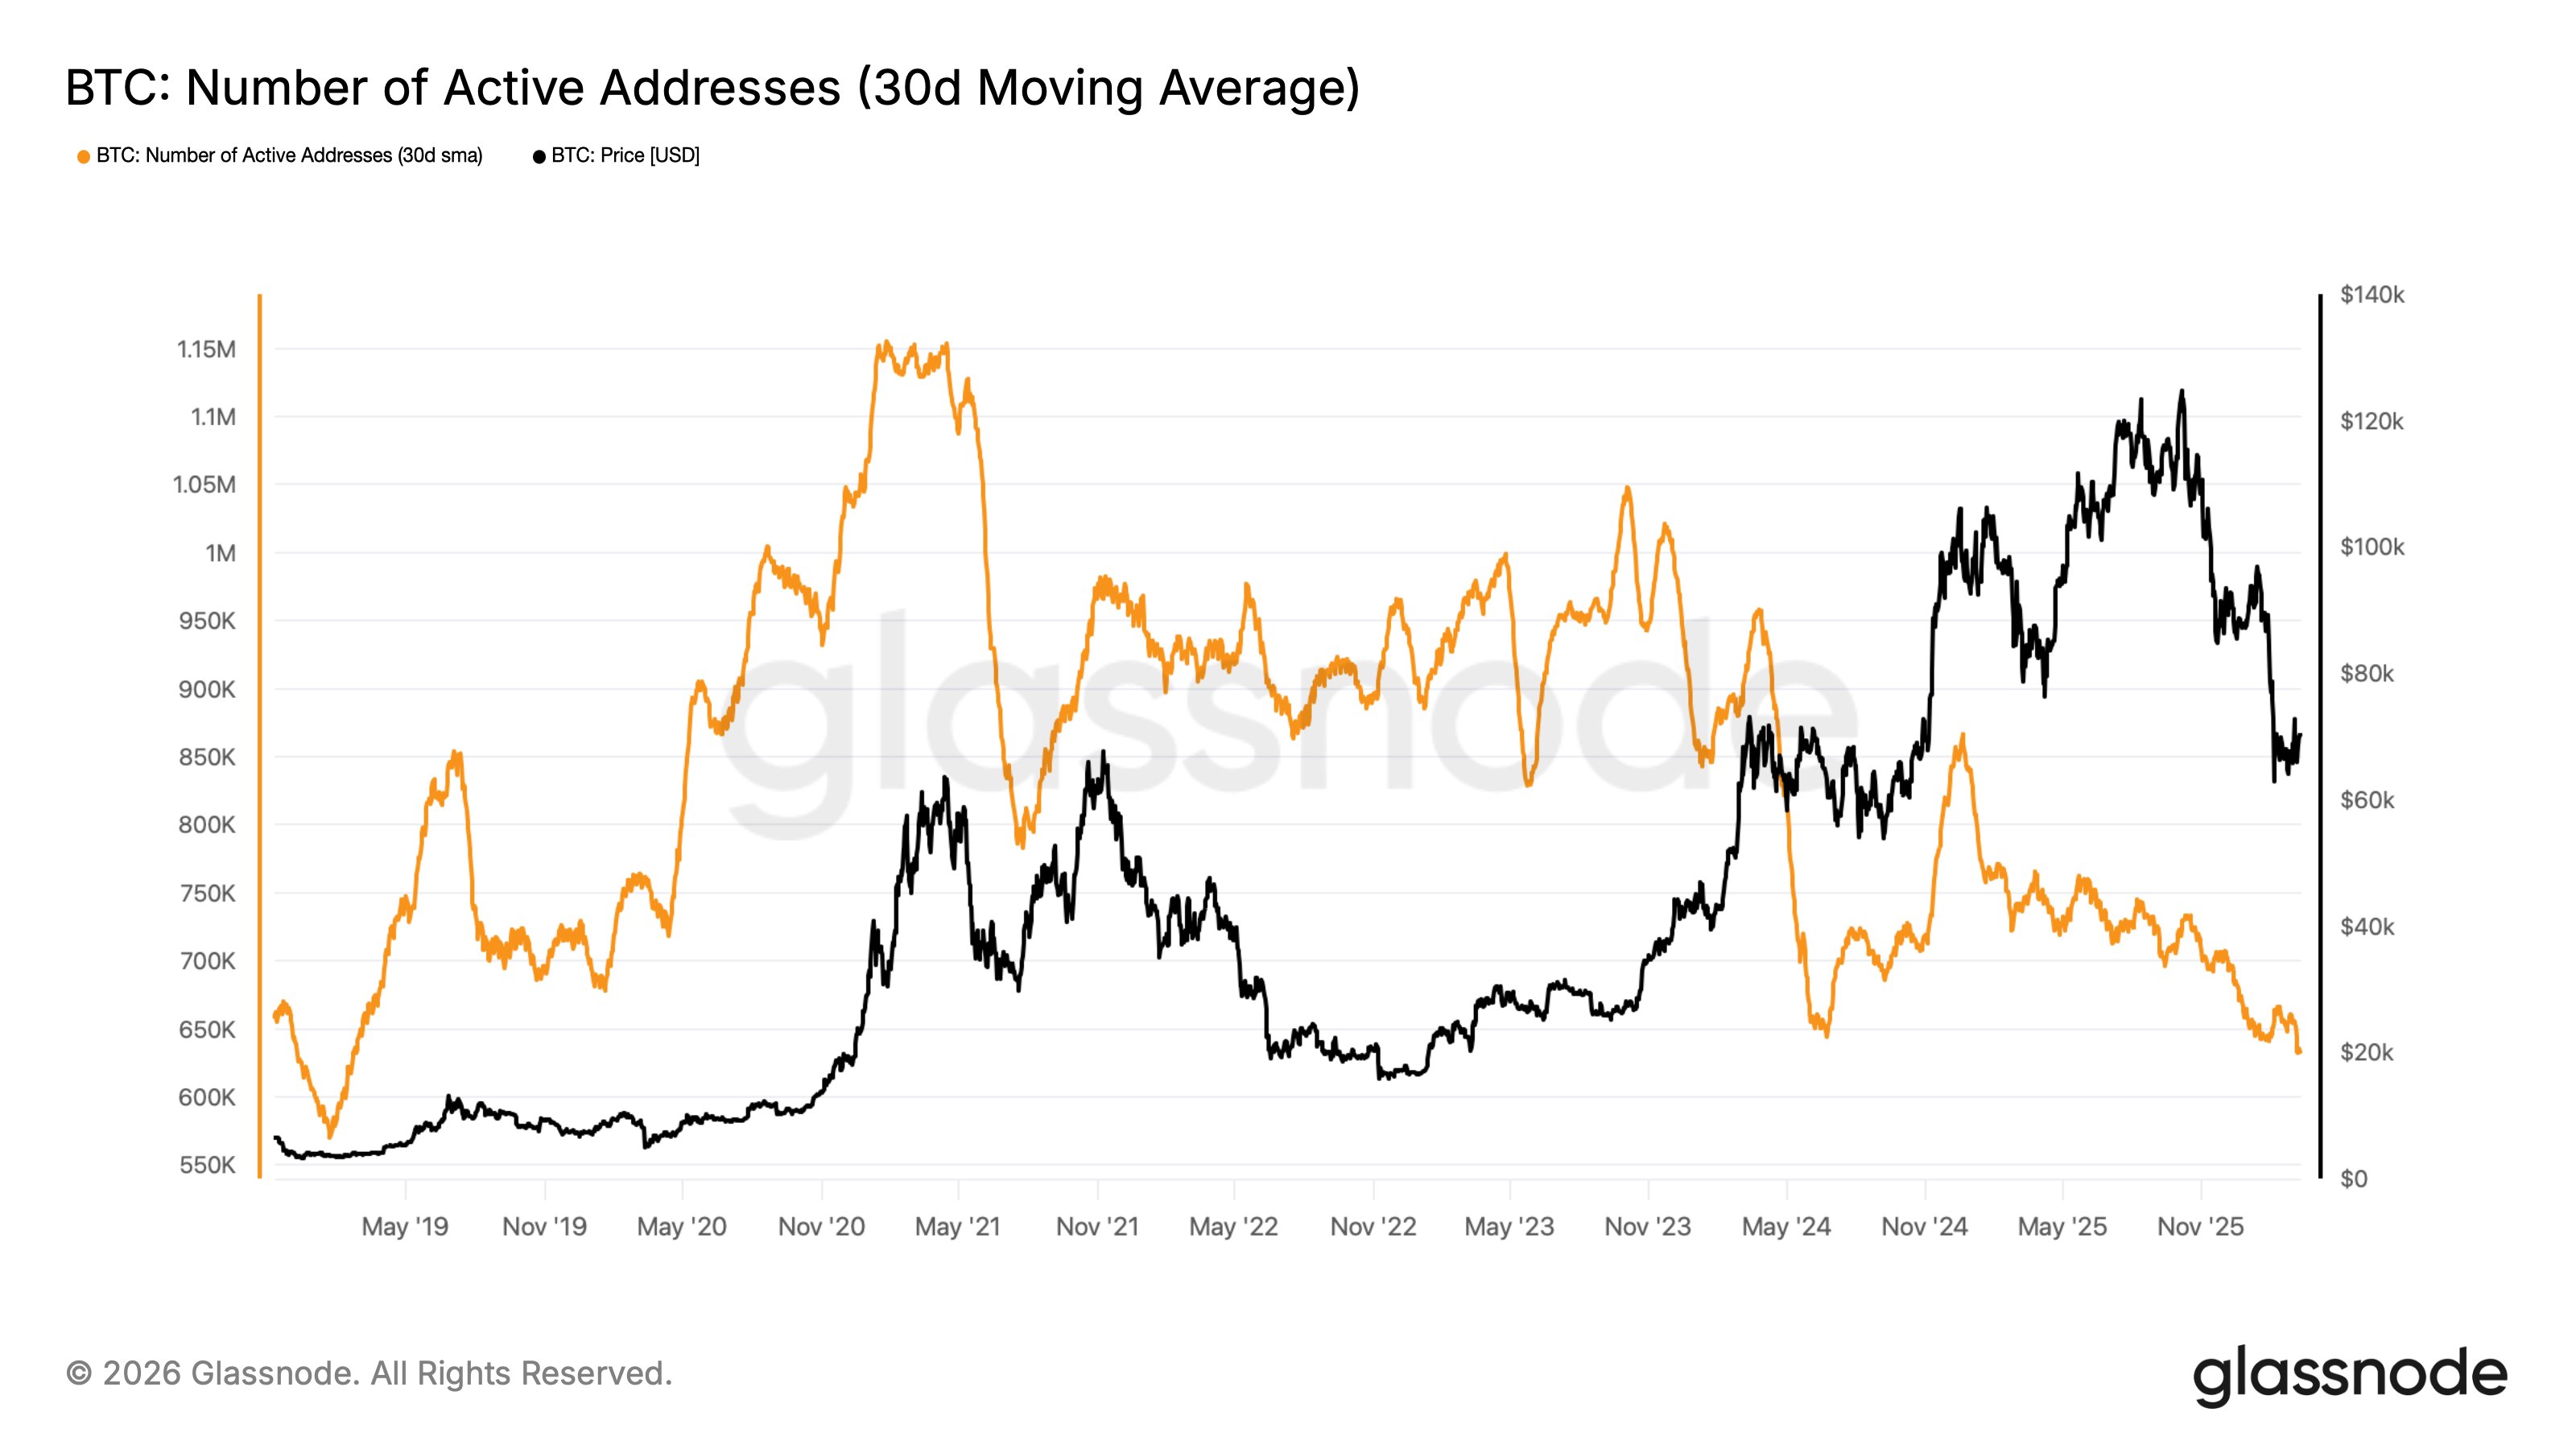
\includegraphics[width=1\linewidth]{Figures/glassnode-studio_btc-number-of-active-addresses-30d-moving-average.png}
\caption{Bitcoin market cap vs.\ active addresses (30d MA). Source: Glassnode}
    \label{fig:active addresses}
\end{figure}
\end{frame}

\begin{frame}{Valuation Framework 2: Stock-to-Flow}
  \textbf{Idea}: Bitcoin's value should be related to its scarcity, measured by the \highlight{stock-to-flow ratio}:
  $$\text{Stock-to-Flow} = \frac{\text{Existing supply}}{\text{Annual new production}}$$
  
  \vspace{0.3em}
  The higher the ratio, the scarcer the asset. Gold has a high stock-to-flow ($\approx 60$); Bitcoin's increases after each halving.
  
  \vspace{0.5em}
  \textbf{The model:} Regress $\log(\text{price})$ on $\log(\text{S2F})$. This produced impressive in-sample fits in early work (PlanB, 2019).
  
  \vspace{0.5em}
  \textbf{Why the model failed:}
  \begin{itemize}
    \item Post-2021, Bitcoin's price significantly underperformed the S2F prediction
    \item The model implies price goes to infinity as flow approaches zero---economically nonsensical
    \item Confuses scarcity with \textit{demand}: scarcity is \textit{necessary} but not \textit{sufficient} for value. Demand matters too---and for crypto, demand is driven by speculation, adoption, and narrative, not by supply schedules alone.
  \end{itemize}
  
\end{frame}

\begin{frame}{Valuation Framework 2: Stock-to-Flow}

 \begin{figure}
    \centering
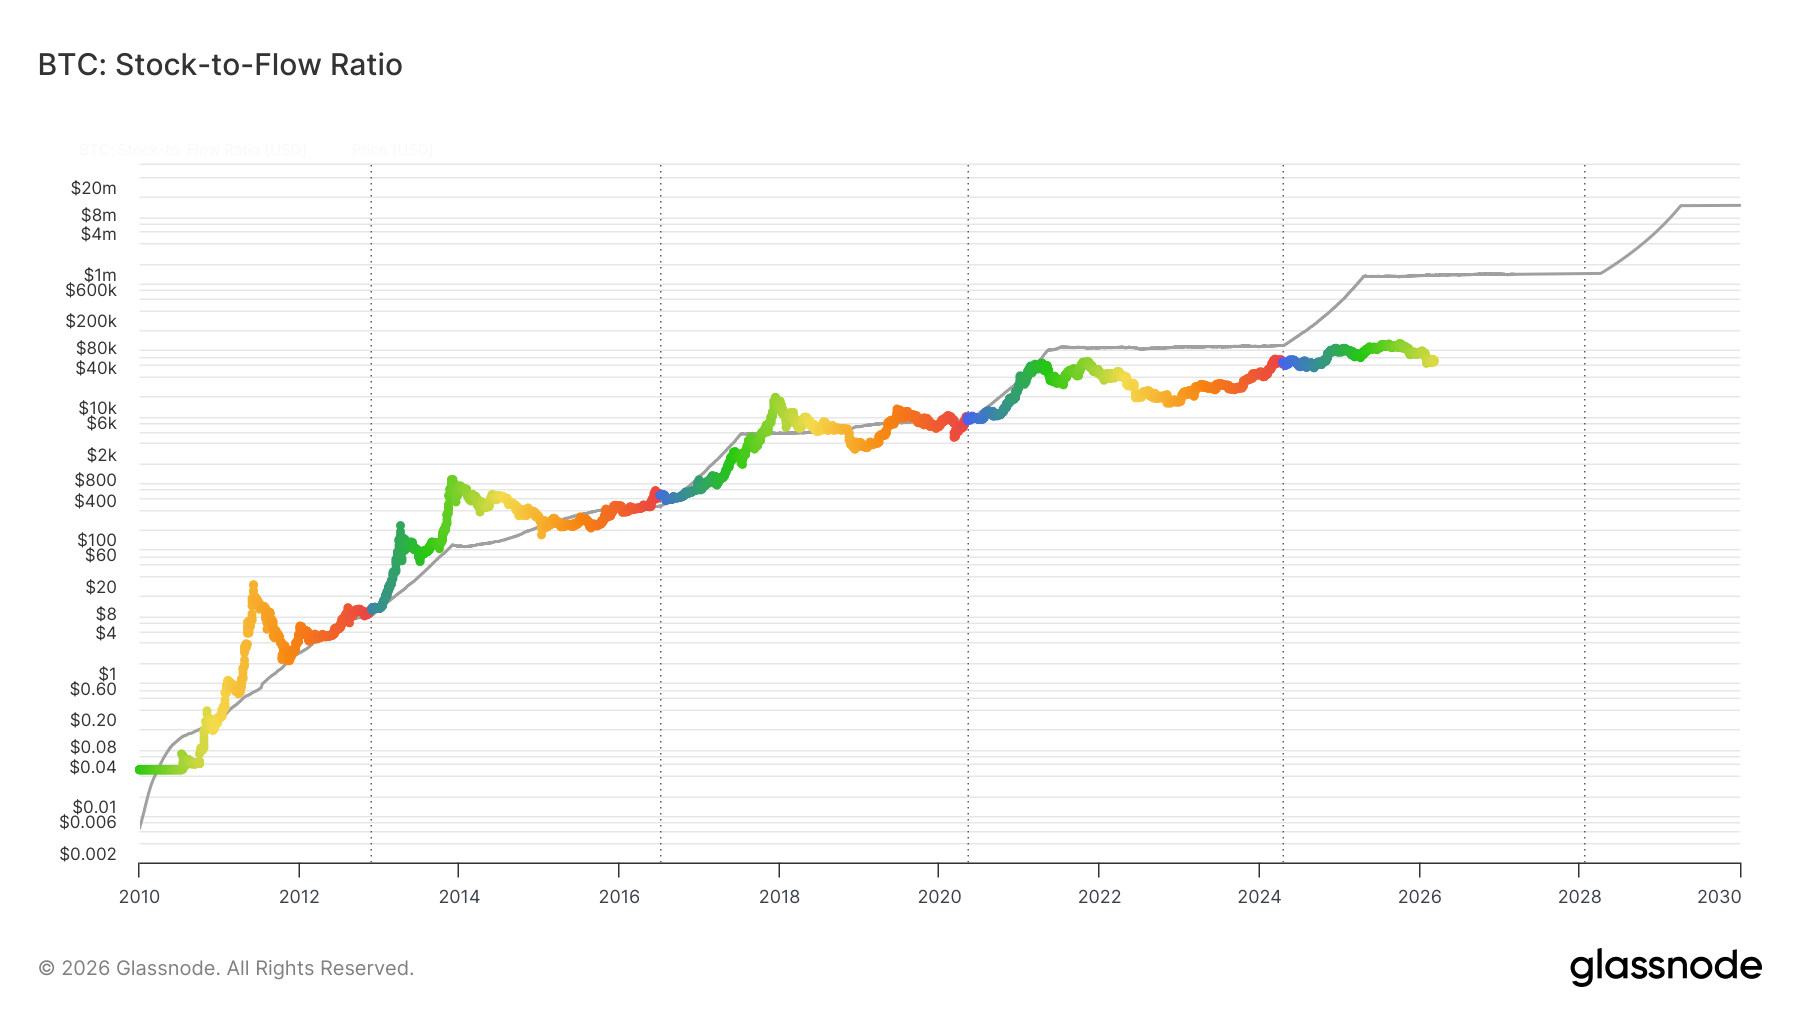
\includegraphics[width=1\linewidth]{Figures/glassnode-studio_btc-stock-to-flow-ratio.png}
\caption{Stock-to-flow is defined as the ratio of the current stock of a commodity (i.e., the circulating Bitcoin supply) to the flow of new production (i.e., newly mined bitcoins). Source: Glassnode}
    \label{fig:s2f}
\end{figure}
\end{frame}

\begin{frame}{Valuation Framework 3: Cost of Production}
  \textbf{Idea}: Bitcoin's ``fundamental value'' is anchored by the cost of mining it.
  
  \vspace{0.5em}
  \textbf{The argument:}
  \begin{itemize}
    \item Mining requires electricity and hardware---real economic costs
    \item Rational miners will not mine at a loss for long
    \item Therefore, the cost of production acts as a price floor
  \end{itemize}
  
  \vspace{0.5em}
  \textbf{Why this is incomplete:}
  \begin{itemize}
    \item Causality runs both ways: higher prices attract more miners, \textit{raising} the cost of production. The cost adjusts to the price, not only the other way around.
    \item Difficulty adjustment ensures block production continues regardless of price or hashrate level
    % \item Many miners operate in locations with subsidised or stranded energy---marginal costs vary enormously
    \item Does not apply to Proof-of-Stake tokens at all
  \end{itemize}
  
  \vspace{0.5em}
  \textbf{Useful insight}: After halvings, less efficient miners are forced out, creating short-term supply pressure. The April 2024 halving reduced the block reward from 6.25 to 3.125 BTC.
\end{frame}

\begin{frame}{Valuation Framework 4: Tokenomics}
  For tokens beyond Bitcoin, \textbf{tokenomics}---the economic design of the token---matters for valuation.
  
  \vspace{0.5em}
  \textbf{Key tokenomics factors:}
  \begin{itemize}
    \item \textbf{Supply schedule}: Fixed (BTC), inflationary (early ETH), deflationary (post-EIP-1559 ETH with fee burning)
    \item \textbf{Token distribution}: How concentrated is ownership? Insider share?
    \item \textbf{Utility}: Is the token \textit{required} to use the protocol? (ETH for gas fees) Or is it purely governance/speculative?
    \item \textbf{Value capture}: Does protocol revenue flow to token holders? (e.g., fee-sharing, buyback-and-burn mechanisms)
  \end{itemize}
  
  \vspace{0.5em}
  \textbf{The ETH case} is instructive:
  \begin{itemize}
    \item Post-Merge: stakers earn $\sim$3--4\% yield (real economic return)
    \item EIP-1559: Base fees are burned, reducing supply
    \item This creates something \textit{closer} to a cash-flow asset
  \end{itemize}
  
  \vspace{0.3em}
  \begin{block}{Bottom Line}
    There is no single ``correct'' crypto valuation model. Investors must combine multiple frameworks and remain honest about uncertainty.
  \end{block}
\end{frame}

%----------------------------------------------------------------------------------------
\section{Risk-Return Characteristics}
%----------------------------------------------------------------------------------------

\begin{frame}{Return Characteristics}
  Cryptocurrency returns have been extraordinary over long horizons, but extremely uneven:
  
  \vspace{0.5em}
  \textbf{Key facts:}
  \begin{itemize}
    \item Bitcoin: $\sim$150\% annualised return since 2013, but with multiple $>$50\% drawdowns
    \item Ethereum: Even higher returns since 2015, with even higher volatility
    \item Most altcoins: The majority have delivered \textit{negative} lifetime returns
  \end{itemize}
  
  \vspace{0.5em}
  \textbf{Survivorship bias warning:} Focusing on BTC and ETH overstates the returns an average crypto investor earned. CoinGecko lists over 13,000 tokens; most are effectively dead.
  
  % \vspace{0.5em}
  % % FIGURE PLACEHOLDER: Two-panel figure
  % % Left: Total crypto market capitalisation over time (2015--2025)
  % % Right: Market cap dominance breakdown (BTC, ETH, stablecoins, others)
  % % Source: CoinGecko
  % \textit{[Figure: Total crypto market cap and dominance breakdown. Source: CoinGecko]}
  
  % \vspace{0.3em}
  % \begin{block}{Interpretation}
  %   High average returns reflect high \highlight{risk compensation}, not free money. We need to examine the risk side carefully.
  % \end{block}
\end{frame}



\begin{frame}{Volatility}
  Crypto volatility is substantially higher than that of traditional asset classes.
  
  \vspace{0.5em}
  \textbf{Typical annualised volatility ranges:}
  \begin{center}
    \small
    \begin{tabular}{lc}
      \toprule
      \textbf{Asset} & \textbf{Annualised volatility (approx.)} \\
      \midrule
      S\&P 500 & 15--20\% \\
      Gold & 12--18\% \\
      Crude Oil & 25--40\% \\
      Bitcoin & 50--80\% \\
      Ethereum & 70--100\% \\
      Typical altcoin & 100--200\%+ \\
      \bottomrule
    \end{tabular}
  \end{center}
  
  \vspace{0.5em}
  \textbf{Important nuance:} Bitcoin's volatility has been \textit{declining} over time as the market matures. 30-day annualised volatility regularly exceeded 100\% before 2020; it has mostly stayed in the 40--70\% range since 2023.
  
  % \vspace{0.5em}
  % % FIGURE PLACEHOLDER: Bitcoin 30-day annualised volatility (2017--2025)
  % % Source: The Block — "Annualized BTC Volatility (30D)"
  % \textit{[Figure: Bitcoin 30-day annualised volatility over time. Source: theblock.co]}
\end{frame}

\begin{frame}{Drawdowns and Tail Risk}
  High volatility is one thing. \highlight{Extreme drawdowns} are another---and crypto has experienced some of the largest in the history of financial markets.
  
  \vspace{0.5em}
  \textbf{Major Bitcoin drawdowns:}
  \begin{center}
    \small
    \begin{tabular}{lcc}
      \toprule
      \textbf{Period} & \textbf{Peak-to-trough} & \textbf{Recovery time} \\
      \midrule
      Dec 2017 -- Dec 2018 & $-$84\% & $\sim$3 years \\
      Apr 2021 -- Jun 2021 & $-$55\% & $\sim$6 months \\
      Nov 2021 -- Nov 2022 & $-$77\% & $\sim$2 years \\
      \bottomrule
    \end{tabular}
  \end{center}
  
  \vspace{0.5em}
  \textbf{For comparison:} The S\&P 500's worst drawdown during the 2008 financial crisis was approximately $-$57\%, and during COVID-19 (March 2020) approximately $-$34\%.
  
  \vspace{0.5em}
  \textbf{Economic implication:} An investor who allocated 10\% of a portfolio to Bitcoin at the November 2021 peak would have seen that position fall to $\sim$2.3\% of portfolio value by November 2022---a loss large enough to meaningfully drag overall portfolio returns.
  
  % \vspace{0.3em}
  % Return distributions for crypto exhibit \textbf{fat tails} and \textbf{negative skewness} during crashes, meaning standard deviation alone underestimates the true risk.
\end{frame}

\begin{frame}{Drawdowns and Tail Risk}
  \begin{figure}
    \centering
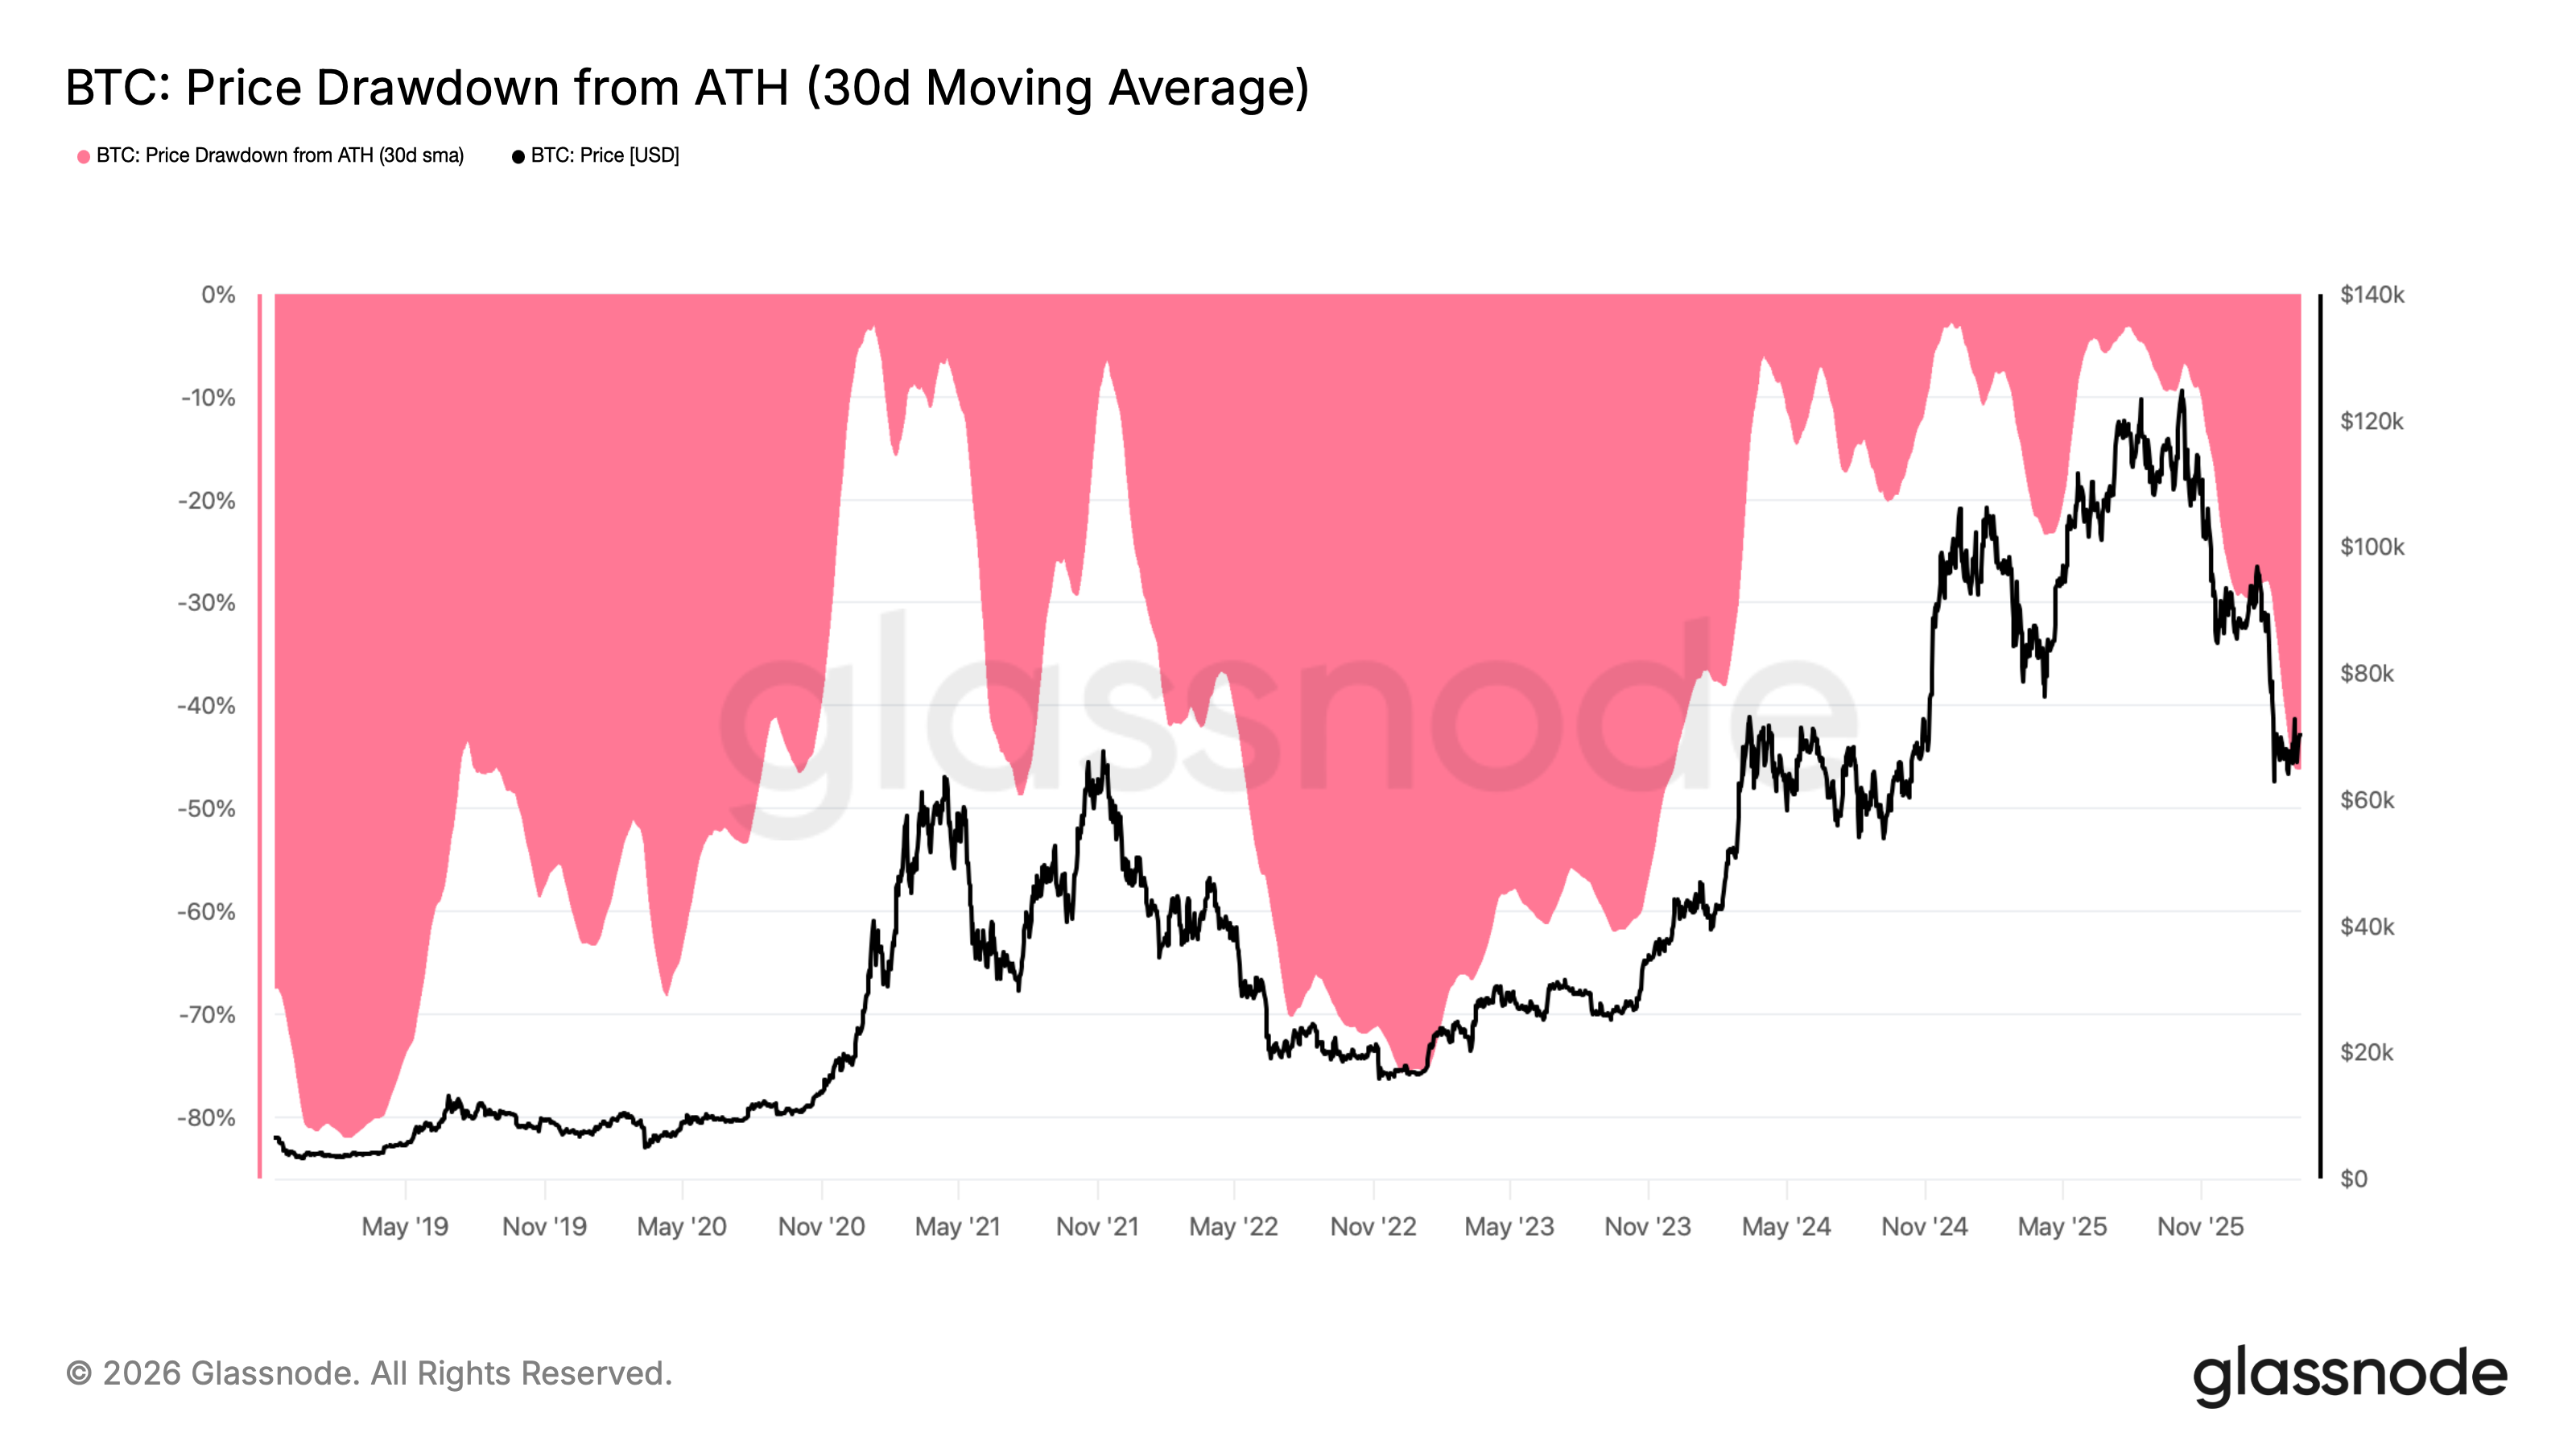
\includegraphics[width=.9\linewidth]{Figures/glassnode-studio_btc-price-drawdown-from-ath-30d-moving-average.png}
\caption{BTC drawdown from all-time high (30d MA). Source: Glassnode}
    \label{fig:s2f}
\end{figure}
  % FIGURE PLACEHOLDER: Two-panel figure
  % Left: Total crypto market capitalisation over time (2015--2025)
  % Right: Market cap dominance breakdown (BTC, ETH, stablecoins, others)
  % Source: CoinGecko
  
  \vspace{0.3em}
  \textbf{Interpretation}: high average returns reflect high \highlight{risk compensation}, not free money. We need to examine the risk side carefully.
\end{frame}

% \begin{frame}{The Sharpe Ratio: Handle with Care}
%   The \textbf{Sharpe ratio} is commonly used to compare risk-adjusted returns across assets:
%   $$\text{Sharpe Ratio} = \frac{\E[R] - R_f}{\sigma(R)}$$
  
%   where $\E[R]$ is the expected return, $R_f$ the risk-free rate, and $\sigma(R)$ the standard deviation.
  
%   \vspace{0.5em}
%   \textbf{Crypto Sharpe ratios look attractive over certain windows}---sometimes exceeding those of equities.
  
%   \vspace{0.5em}
%   % FIGURE PLACEHOLDER: Sharpe ratios across asset classes (trailing 1-year and 3-year)
%   % Source: IntoTheBlock or compute from CoinGecko/Yahoo Finance data
%   % Suggestion: Show both a favourable window and an unfavourable one
%   \textit{[Figure: Sharpe ratios across asset classes for different time windows. Source: IntoTheBlock / Yahoo Finance]}
  
%   \vspace{0.5em}
%   \textbf{Why you should be cautious:}
%   \begin{itemize}
%     \item Sharpe ratios assume normally distributed returns---crypto returns are \textit{not} normal (fat tails, skewness)
%     \item Extremely sensitive to the sample period chosen
%     \item A 1-year window starting January 2023 looks excellent; one starting November 2021 looks terrible
%     \item For fat-tailed distributions, the \textbf{Sortino ratio} (penalising only downside volatility) may be more informative
%   \end{itemize}
% \end{frame}

\begin{frame}{Correlation with Traditional Assets}
  \textbf{The diversification argument:} If crypto returns are uncorrelated with equities and bonds, even a small allocation improves portfolio efficiency (higher return per unit of risk).
  
  \vspace{0.5em}
  \textbf{What the data shows:}
  \begin{itemize}
    \item Pre-2020: BTC-S\&P 500 correlation was near zero on average---consistent with the diversification narrative
    \item 2020--2022: Correlation spiked significantly during COVID and the subsequent tightening cycle, reaching 0.5--0.7 at times
    \item 2023--2025: Correlation has moderated but remains higher than the pre-2020 baseline
  \end{itemize}
  
  % \vspace{0.5em}
  % % FIGURE PLACEHOLDER: BTC 30-day rolling correlation with S&P 500, Nasdaq, and Gold
  % % Source: The Block — "BTC Pearson Correlation (30D)"
  % \textit{[Figure: BTC rolling 30-day correlation with equities and gold. Source: theblock.co]}
  
  % \vspace{0.5em}
  % \begin{block}{Key Insight}
  %   Correlations are \highlight{time-varying} and tend to \highlight{increase during crises}---precisely when diversification is most needed. This is a well-known phenomenon in finance (correlation breakdown), and crypto is not exempt.
  % \end{block}
\end{frame}

\begin{frame}{Correlation with Traditional Assets}


   \begin{figure}
    \centering
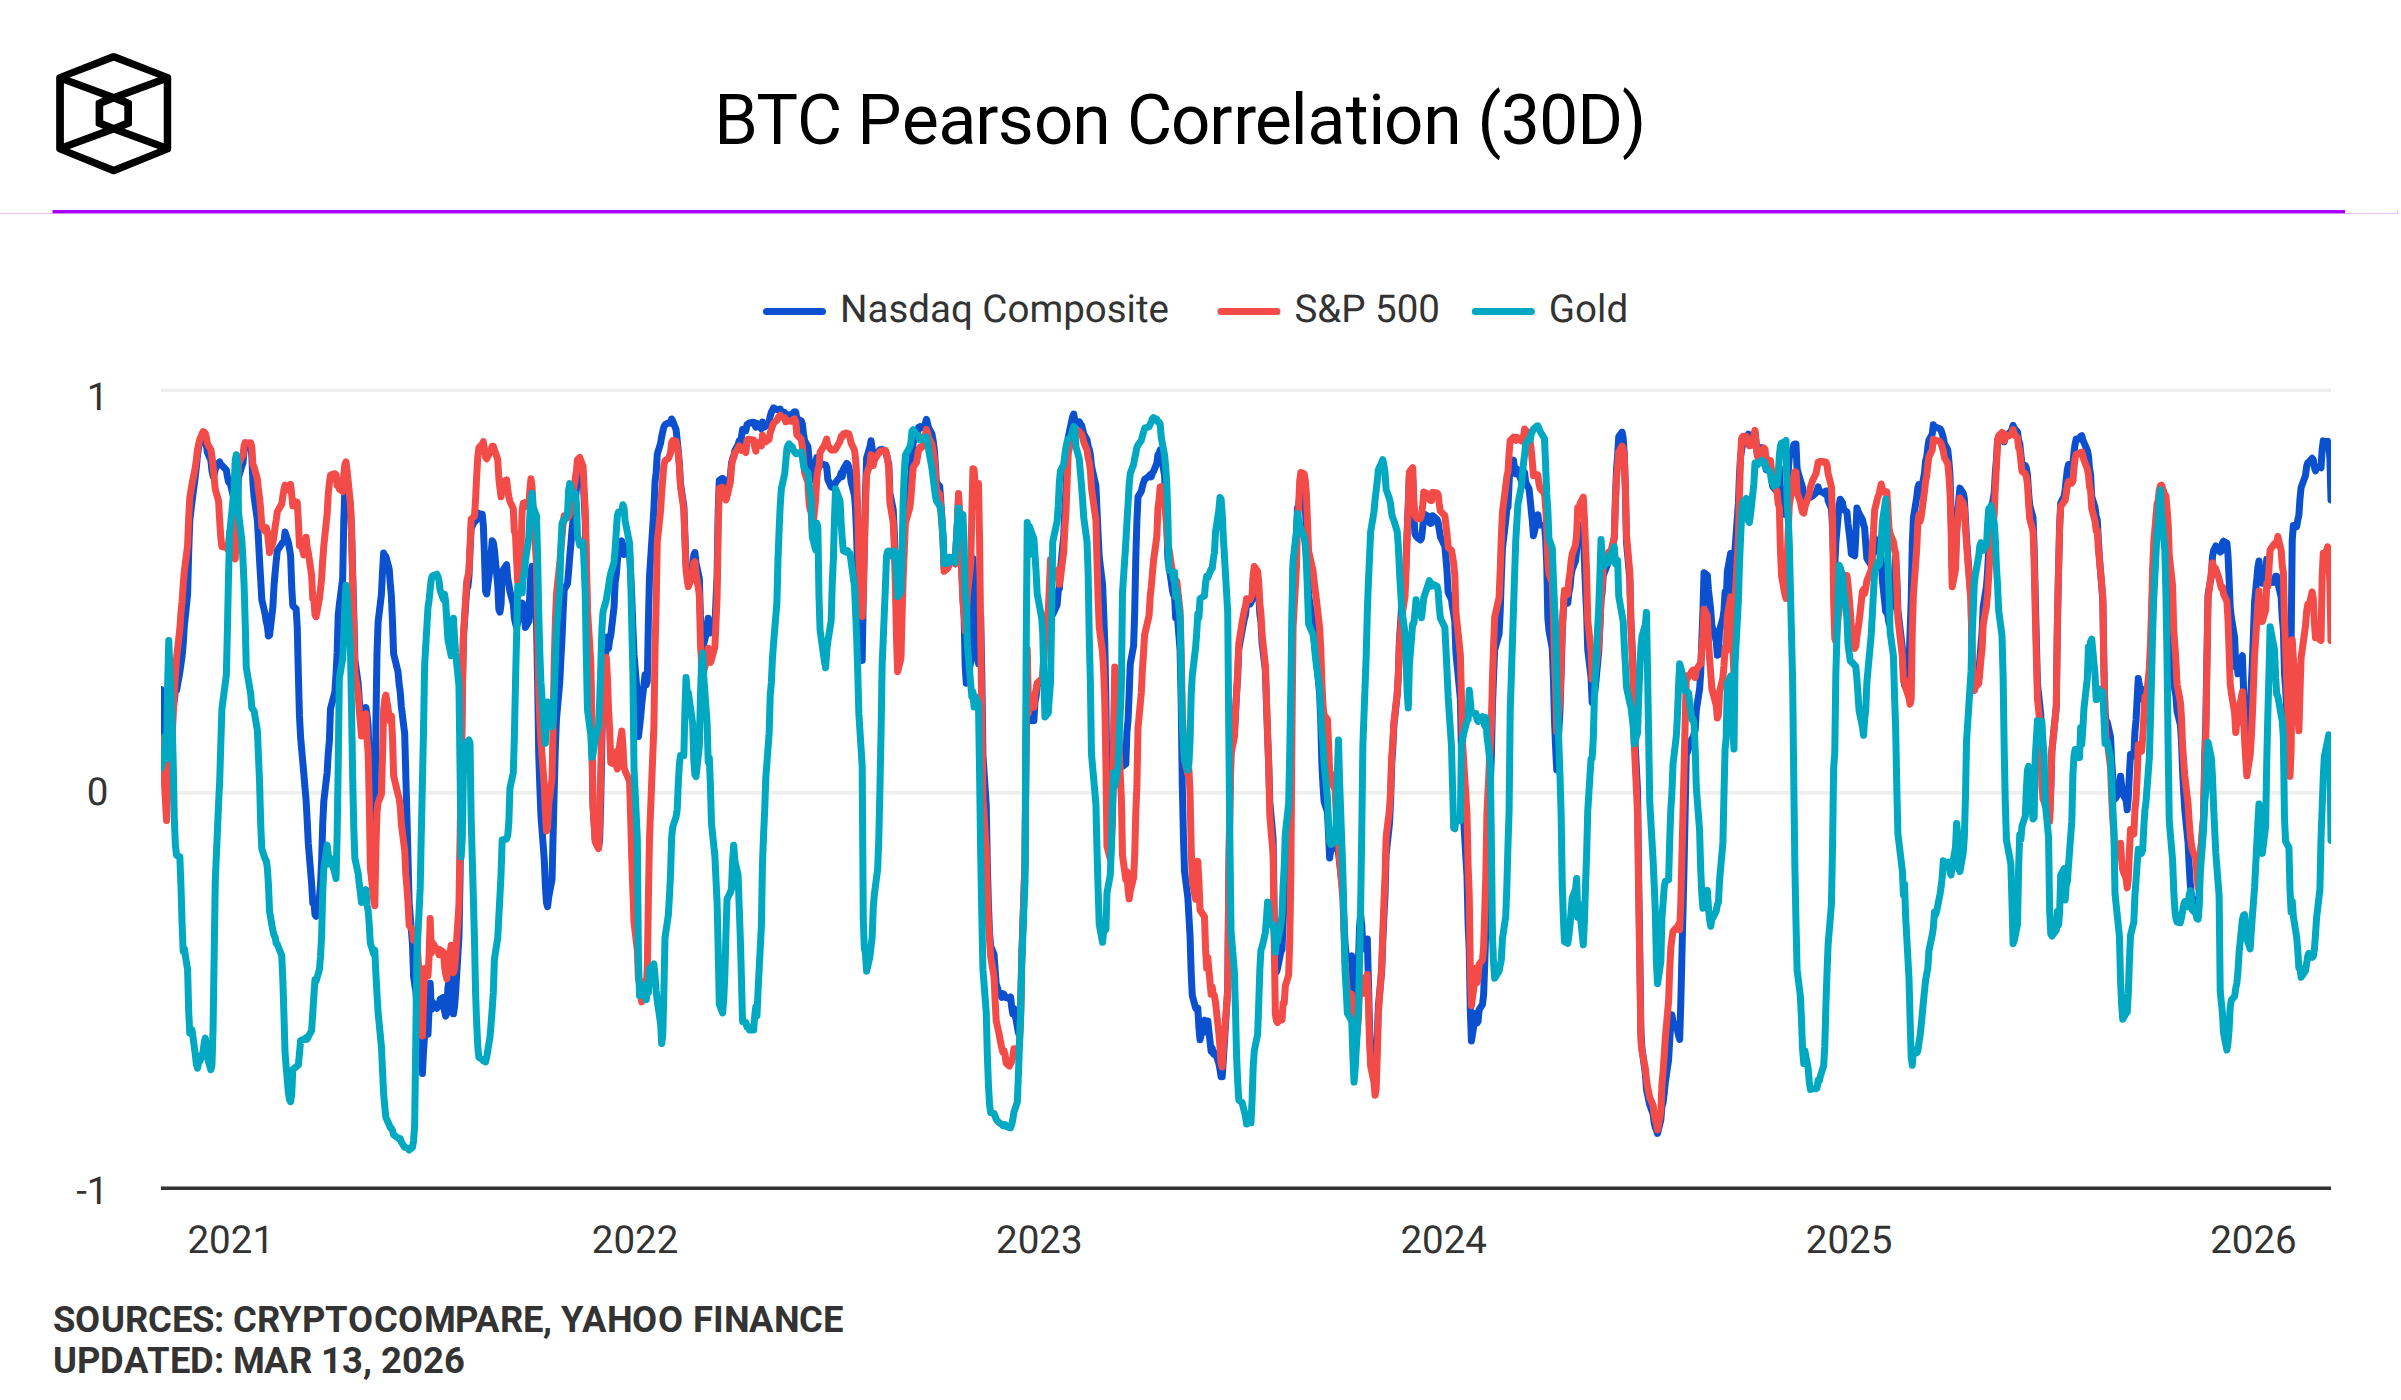
\includegraphics[width=.9\linewidth]{Figures/btc-pearson-correlation-30d.png}
\caption{BTC rolling 30-day correlation with equities and gold. Source: theblock.co}
    \label{fig:correlation}
\end{figure}
  
  % \vspace{0.5em}
  % \begin{block}{Key Insight}
  %   Correlations are \highlight{time-varying} and tend to \highlight{increase during crises}---precisely when diversification is most needed. This is a well-known phenomenon in finance (correlation breakdown), and crypto is not exempt.
  % \end{block}
\end{frame}

\begin{frame}{Why Did Correlations Increase?}
  The rise in BTC-equity correlation after 2020 is not accidental. Several structural factors explain it:
  
  \vspace{0.5em}
  \begin{enumerate}
    \item \textbf{Institutional participation}: As hedge funds, family offices, and asset managers entered crypto, the same portfolio rebalancing flows that move equities now also move Bitcoin.
        
    \vspace{0.3em}
    \item \textbf{Risk-on / risk-off dynamics}: In a flight to safety, investors sell \textit{all} risky assets---crypto included. In a risk-on environment, liquidity flows into \textit{all} risky assets.
    
    \vspace{0.3em}
    \item \textbf{Leverage}: Leveraged positions in crypto are often funded with the same capital that funds equity positions. Margin calls force simultaneous liquidation.
  \end{enumerate}
  
  \vspace{0.5em}
  \textbf{Implication for portfolio construction}: The ``uncorrelated alpha'' argument for crypto has weakened. Crypto may still offer diversification at certain frequencies or horizons, but it is not a reliable hedge against equity drawdowns.
\end{frame}

\begin{frame}{What About Bitcoin as ``Digital Gold''?}
  A popular narrative positions Bitcoin as a \highlight{store of value} and \highlight{inflation hedge}, analogous to gold.
  
  \vspace{0.5em}
  \textbf{Arguments in favour:}
  \begin{itemize}
    \item Fixed supply (21 million cap) vs.\ fiat money printing
    \item Not controlled by any government or central bank
    \item Portable, divisible, verifiable
  \end{itemize}
  
  \vspace{0.5em}
  \textbf{What the evidence shows:}
  \begin{itemize}
    \item During the 2021--2023 inflation episode, Bitcoin \textit{fell} while inflation rose---inconsistent with an inflation hedge
    \item BTC-Gold correlation is low and unstable (sometimes positive, sometimes negative)
    \item Bitcoin's volatility ($\sim$60\%) is roughly 4$\times$ that of gold ($\sim$15\%)---a very ``noisy'' store of value
  \end{itemize}
  
  % \vspace{0.5em}
  % \begin{block}{Assessment}
  %   Bitcoin may \textit{eventually} function as digital gold if volatility continues to decline and adoption broadens. But the empirical evidence as of 2025 does not support this claim---it remains a narrative, not a fact.
  % \end{block}
\end{frame}

%----------------------------------------------------------------------------------------
\section{Summary and Next Steps}
%----------------------------------------------------------------------------------------

\begin{frame}{Key Takeaways}
  \begin{enumerate}
    \item \textbf{Crypto markets are structurally different from traditional markets}
    \begin{itemize}
      \item Fragmented, 24/7, varying regulation, custody is a first-order problem
    \end{itemize}
    
    \vspace{0.3em}
    \item \textbf{Valuation is fundamentally challenging}
    \begin{itemize}
      \item No cash flows for most tokens; alternative frameworks (network value, S2F, cost of production) are suggestive but not reliable
      \item Tokenomics and utility provide partial anchors for some assets (ETH)
    \end{itemize}
    
    \vspace{0.3em}
    \item \textbf{Returns have been high but so has risk}
    \begin{itemize}
      \item Extreme volatility, large drawdowns, fat-tailed distributions
      \item Sharpe ratios are sample-dependent and misleading for non-normal returns
    \end{itemize}
    
    \vspace{0.3em}
    \item \textbf{The diversification benefit is weaker than advertised}
    \begin{itemize}
      \item Correlations with equities increased post-2020
      \item ``Digital gold'' narrative not supported by inflation-episode evidence
    \end{itemize}
    
    \vspace{0.3em}
    \item \textbf{None of this means crypto is uninvestable}---but it means investors need to go in with clear eyes about what they are buying and why
  \end{enumerate}
\end{frame}

\begin{frame}{What's Next}
  \textbf{Week 8: Cryptocurrencies as an Asset Class (Part II)}
  \begin{itemize}
    \item The 2024 Bitcoin and Ethereum spot ETF approvals
    \item How ETFs work: structure, fees, flows, and price discovery
    \item The regulatory battle that made ETFs possible (SEC, Grayscale)
    \item Institutional adoption: custody solutions, prime brokerage, corporate treasuries
    \item Investment vehicles: direct, indirect, and derivatives
    \item Market manipulation and integrity risks
  \end{itemize}
  
  \vspace{1em}
  \textbf{Preparation:}
  \begin{itemize}
    \item Think about: Why did the SEC resist approving a Bitcoin spot ETF for over a decade? What changed?
    \item Explore: Look up the current AUM of the iShares Bitcoin Trust (IBIT) and compare it to major gold ETFs
  \end{itemize}
\end{frame}

\begin{frame}[plain]
  \vfill
  \begin{center}
    {\Large Questions?}
  \end{center}
  \vfill
\end{frame}

\end{document}